\documentclass{article}

%%package
\usepackage{amsmath}
\usepackage{amssymb}
\usepackage{amsthm}
\usepackage{palatino}
\usepackage{tikz}

%% def
\newcommand{\atoms}{\textsf{\small{At}}}
\newcommand{\actions}{\Sigma}
\newcommand{\bisim}[1]{\sim_{#1}}
\newcommand{\mat}[1]{\textbf{Mat}(#1)}
\newcommand{\gs}{\textbf{GS}}


\newcommand{\terms}{T_{K,F_n}}
\newcommand{\universe}{(2^{\atoms\times\atoms})^\gs}
\newcommand{\coproduct}{K \oplus F_n / D}

\newcommand{\todo}[1]{\textbf{TODO:~#1}}

\newtheorem{corollary}{Corollary}
\newtheorem{lemma}{Lemma}

%% main
\begin{document}

\section*{Coalgebraic Decision Procedure for KAT + B!}

\subsection*{One}

The original KAT+B! paper shows that an arbitrary KAT+B! is isomorphic to the family of matrices $\mat{\atoms,K}$.

The set $\atoms$ are the elements of the boolean algebra B!.
The set $K$ is the KAT.
The matrices are all of dimension $\atoms \times \atoms$ and contain elements of $K$ in their cells.
(In other words, $(\atoms \times \atoms)$-indexed elements of $K$.)

%% This isomorphism is partially made possible by an injection from B! to its language model $2^{\atoms \times \atoms}$.
%% It is $(\atoms \times \atoms)$ because the B! algebra permits tests and assignments.
%% But that's not so important to the current discussion.

We also have an injection from any KAT into the language model of KATs.
The language model for KATs is the set of all guarded strings over elements of $K$, so we have the injection $KAT \hookrightarrow 2^\gs$ (specifically, guards are from the embedded boolean algebra of the KAT and strings are from the set of actions $\actions$~of the KAT).

Applying this injection \todo{how, exactly? pointwise?} to the family $\mat{\atoms,K}$, we get an injection $\mat{\atoms,K} \hookrightarrow \mat{\atoms,2^\gs}$.
Great!
From here we can apply currying to morph $\mat{\atoms,2^\gs}$ to $\mat{\gs,\mat{\atoms,2}}$.
Alternatively, $\mat{\gs,\mat{\atoms,2}}$ may be written as $(2^{\atoms\times\atoms})^\gs$.
From here on, let $U = \universe$.

\todo{Introduce commutative coproduct $(K + F_n) / D \cong \mat{2^n,K}$}

Let $I : \coproduct \hookrightarrow U$ denote the injection we have just constructed.

Lastly, we have an isomorphism $h : T_{k,F_u} \rightarrow \coproduct$ taking terms from the \todo{what are terms} to the commutative coproduct defined by the KAT+B!.

\subsection*{Two}

Let $\atoms$~now refer to the elements on the embedded boolean algebra of KAT.
(We assume the elements of the complete boolean algebra B! are indexed in $F_n$.)

Want to find an $F X = (2^{2n})^\atoms \times X^{\atoms\actions}$ \todo{describe F}

Need to prove two lemmas:

\begin{lemma}
  $U$ is final F-coalgebra.
  If $L,K \in U$ and $L \bisim{F} K$ then $L = K$.
\end{lemma}
\begin{proof}
  todo
\end{proof}

\begin{lemma}
  The unique F-coalgebra homomorphism satisfies $u = G = I \circ h$
\end{lemma}
\begin{proof}
  First, we restate definitions.
  The arrow $u : \terms \rightarrow U$ takes terms to the universe $\universe$.
  The arrow $h : \terms \rightarrow \coproduct$ takes terms to the commutative coproduct of KAT+B!.
  Lastly the arrow $I : \coproduct \rightarrow U$ is the injection from the coproduct to the universe.

  We want to prove that the arrow $u$ is unique in the following commutative diagram.
  \begin{center}
    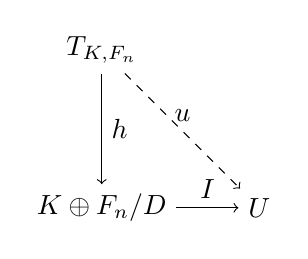
\begin{tikzpicture}
      \node (1) {$\terms$};
      \node [below of=1,yshift=-1cm] (2) {$\coproduct$};
      \node [right of=2,xshift=1cm] (3) {$U$};

      \draw[dashed,->] (1) -- node[above] {$u$} (3);
      \draw[->] (1) -- node[right] {$h$} (2);
      \draw[->] (2) -- node[above] {$I$} (3);
    \end{tikzpicture}
  \end{center}
  
\end{proof}

The result of these lemmas is the following corollary:
\begin{corollary}
  If $R \subseteq \terms \times \terms$ is an F-bisimulation and $(p,q) \in R$ then KAT+B! $\vDash p = q$
\end{corollary}

\subsection*{Tools}

\subsubsection*{Bisimilarity}

A relations $R \subseteq X \times X$ is an F-bisimulation if for all $(x,y) \in R$, it holds:
\begin{enumerate}
\item $\varepsilon(x) = \varepsilon(y)$
\item $\forall \alpha \in \atoms,~ \rho \in \actions~.~(\delta_{\alpha,\rho}(x), \delta_{\alpha,\rho}(y)) \in R$
\end{enumerate}

\subsubsection*{Bigger Picture}

This diagram is important for the lemmas
\begin{center}
  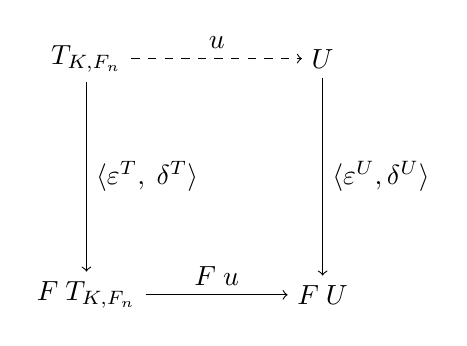
\begin{tikzpicture}
    \node (1) {$\terms$};
    \node[right of=1,xshift=2cm] (2) {$U$};
    \node[below of=1,yshift=-2cm] (3) {$F~T_{K,F_n}$};
    \node[right of=3,xshift=2cm] (4) {$F~U$};

    \draw[dashed,->] (1) -- node[above] {$u$} (2);
    \draw[->] (1) -- node[right] {$\langle \varepsilon^T,~\delta^T\rangle$} (3);
    \draw[->] (2) -- node[right] {$\langle \varepsilon^U,\delta^U \rangle$} (4);
    \draw[->] (3) -- node[above] {$F~u$} (4);
  \end{tikzpicture}
\end{center}

\end{document}
